\documentclass[../thesis.tex]{subfiles}
\begin{document}

\chapter{Simulation model}
\label{chp:model}

Within this part the creation process of the simulation model will be explained in greater detail. At first the three basic equations the software solves will be given followed by a brief overview of the steps taken to create the model. Then the model's results are explained and compared to already done experiments for validation.

\section{governing equations}
\label{sec:gov_eqn}
To obtain the results of interest the model needs to solve three different equations that are linked to each other.

\subsection{mass conservation}
To gain information about the velocity field the mass conservation equations for mass and momentum needs to solved. For 2D axisymmetric case as used here the equations looks like this \cite{manual2009ansys}:

\begin{equation}
	\label{eqn:ansys_conti}
	\dfrac{\partial \rho}{\partial t} + \dfrac{\partial}{\partial x} (\rho u_x) + \dfrac{\partial }{\partial r} (\rho u_r)
	+ \dfrac{\rho u_r}{r} = S_m
\end{equation}

This is the continuity equation where $r$ is the radial coordinate, $u_x$ is the axial velocity, $u_r$ is the radial velocity, $\rho$ is the density and $S_m$ is the source term. In addition to the shown continuity equation the radial and axial momentum equations need to be solved.

%\begin{equation}
%	\dfrac{\partial}{\partial t}(\rho u_x) + \dfrac{1}{r} \dfrac{\partial}{\partial x}(r \rho u_x^2)
%	+ \dfrac{1}{r} \dfrac{\partial}{\partial r}(r \rho u_r u_x) = 
%	- \dfrac{\partial p}{\partial x} + \dfrac{1}{r} \dfrac{\partial }{\partial x} \left[ 
%		r \mu \left( 2 \dfrac{\partial u_x}{\partial x} - \dfrac{2}{3}(\nabla \cdot \mathbf{u}) \right)
%	\right] + \dfrac{1}{r} \dfrac{\partial }{\partial r} \left[ 
%	r \mu \left( \dfrac{\partial u_x}{\partial r} - \dfrac{\partial u_r}{\partial x} \right)
%	\right]
%\end{equation}

\begin{gather}
	\dfrac{\partial}{\partial t}(\rho u_x) + \dfrac{1}{r} \dfrac{\partial}{\partial x}(r \rho u_x^2)
	+ \dfrac{1}{r} \dfrac{\partial}{\partial r}(r \rho u_r u_x) = 
	- \dfrac{\partial p}{\partial x} + \dfrac{1}{r} \dfrac{\partial }{\partial x} \left[ 
	r \mu \left( 2 \dfrac{\partial u_x}{\partial x} - \dfrac{2}{3}(\nabla \cdot \mathbf{u}) \right)
	\right] + \\ \nonumber
	\dfrac{1}{r} \dfrac{\partial }{\partial r} \left[ 
	r \mu \left( \dfrac{\partial u_x}{\partial r} - \dfrac{\partial u_r}{\partial x} \right)
	\right]	
\end{gather}

%\begin{equation}
%	\dfrac{\partial}{\partial t}(\rho u_r) + \dfrac{1}{x} \dfrac{\partial}{\partial r}(r \rho u_x u_r)
%	+ \dfrac{1}{r} \dfrac{\partial}{\partial x}(r \rho u_r^2) = 
%	- \dfrac{\partial p}{\partial r} + \dfrac{1}{r} \dfrac{\partial }{\partial x} \left[ 
%	r \mu \left( \dfrac{\partial u_r}{\partial x} - \dfrac{\partial u_x}{\partial r} \right)
%	\right]
%	+ \dfrac{1}{r} \dfrac{\partial }{\partial r} \left[ 
%	r \mu \left( 2 \dfrac{\partial u_r}{\partial r} - \dfrac{2}{3}(\nabla \cdot \mathbf{u}) \right)
%	\right] -
%	2 \mu \dfrac{u_r}{r^2}+ \dfrac{2}{3} \dfrac{\mu}{r}(\nabla \cdot \mathbf{u}) + \rho \dfrac{u_z^2}{r} + %F_r
%\end{equation}

\begin{gather}
	\dfrac{\partial}{\partial t}(\rho u_r) + \dfrac{1}{x} \dfrac{\partial}{\partial r}(r \rho u_x u_r)
	+ \dfrac{1}{r} \dfrac{\partial}{\partial x}(r \rho u_r^2) = 
	- \dfrac{\partial p}{\partial r} + \dfrac{1}{r} \dfrac{\partial }{\partial x} \left[ 
	r \mu \left( \dfrac{\partial u_r}{\partial x} - \dfrac{\partial u_x}{\partial r} \right)
	\right] \\ \nonumber
	+ \dfrac{1}{r} \dfrac{\partial }{\partial r} \left[ 
	r \mu \left( 2 \dfrac{\partial u_r}{\partial r} - \dfrac{2}{3}(\nabla \cdot \mathbf{u}) \right)
	\right] -
	2 \mu \dfrac{u_r}{r^2}+ \dfrac{2}{3} \dfrac{\mu}{r}(\nabla \cdot \mathbf{u}) + \rho \dfrac{u_z^2}{r} + F_r
\end{gather}
The viscosity $\mu$ and the swirl velocity $u_z$ play a role within the momentum equations in extend to the known variables from \autoref{eqn:ansys_conti}.
Within all previous stated equations the product of $\nabla$ and $\mathbf{u}$ can be written as:

\begin{equation}
	\nabla \cdot \mathbf{u} = \dfrac{\partial u_x}{\partial x} + \dfrac{\partial u_r}{\partial r}+ \dfrac{u_r}{r}
\end{equation}
 

\subsection{energy equation}

The energy equation mostly influences the temperature and internal energy of the mixture. The equation the software solves can be written as:

\begin{equation} 
	\frac{\partial}{\partial t} (\alpha_q \rho_q h_q ) + \nabla \cdot (\alpha_q \rho_q \vec u_q h_q )   = \alpha_q \frac{\partial p_q}{\partial t} + \overline{\overline{\tau}}_q : \nabla \vec u_q - \nabla \cdot \vec q_q + S_q + \sum_{p=1}^n (Q_{pq}  + \dot{m}_{pq} h_{pq} - \dot{m}_{qp} h_{qp}) 
\end{equation}

In this equation $\alpha$ describes the non-dimensional Helmholtz-Energy, $h$ is the enthalpy, $u$ is the velocity, $\tau$ is the stress vector and $S_q$ is a enthalpy source. Enthalpy is created by a reaction for example. Additionally the heat fluxes vector $ \vec q$, the heat transfer between different phases $Q$ using the mass transfer rates between phases are used in this equation. The subscripts $q$ stand for all different species needed to be taken into account. 

\subsection{reaction equation}

Since the reaction $ A + B \rightarrow C$ takes place where the two educts $A$ and $B$ meet the amount of product formed needs to calculated for the hole domain. The method used is to calculate the reaction rate, that is dependent of the temperature and species parameters. This rate is then used to calculate the formed product. Within this work the reaction takes place only in one direction so no backwards reaction constants are needed. The reaction rate can be calculated using this equation \cite{manual2009ansys}:

\begin{equation}
	\label{eqn:reaction}
	\hat{R}_{i,r} = {\Gamma} \left(\nu''_{i,r} - \nu'_{i,r} \right) \left(k_{f,r} \prod_{j=1}^{N} \left[C_{j,r} \right]^{(\eta'_{j,r} + \eta''_{j,r})} \right) 
\end{equation}

$\hat{R}_{i,r}$ is the reaction rate, $\nu''_{i,r}$ and $\nu'_{i,r}$ are the stoichiometric numbers of the product and educts, $k_{f,r}$ is the rate constant for the forward reaction, $C_{j,r}$ is the molar concentration of the species $j$ and $\eta'_{j,r} + \eta''_{j,r}$ are the rate exponents and define the reaction order. 
The index $r$ loops through all reactions, in case there is more than one present. The index $j$ is used to distinguish between different species taking part in the reaction.

\section{model setup}
\label{sec:mod_setup}

In this section the steps needed to create the model within \texttt{ANSYS FLUENT} are explained.

\subsection{geometry creation}

Every \texttt{ANSYS FLUENT} model starts with the geometry creation step. This geometry can either be created using the tools \texttt{ANSYS FLUENT} provides it self or be imported from an already existing CAD model. Within this work the geometry is created using ANSYS DesignModeler. In \autoref{fig:ansys_design} the designed model is shown and the used dimensions are listed in \autoref{tab:ansys_design}.

\begin{figure}[htbp]
	\centering
	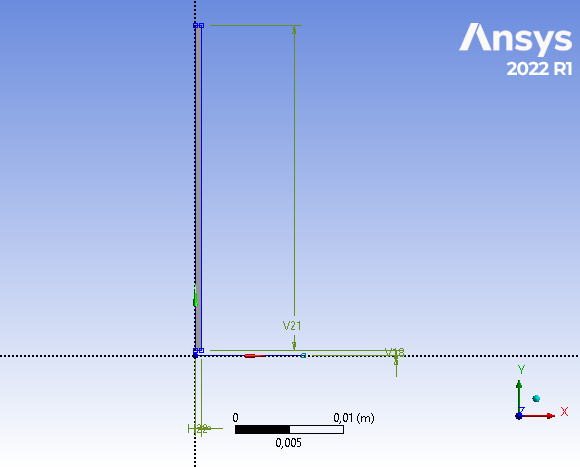
\includegraphics[scale=0.55]{DesignModeler}
	\caption{Geometry Design with Ansys DesignModeler}
	\label{fig:ansys_design}
\end{figure}

\begin{table} [htb]
	\centering
	\caption{Ansys DesignModeler dimensions for geometry example}
	\begin{tabular}{ ccc }
		\hline
		variable & value & unit \\
		\hline
		V21 & 30.0 & mm \\
		V18 & 0.5 & mm \\
		H22 & 0.6 & mm \\
		\hline
		\label{tab:ansys_design}
	\end{tabular}
\end{table}

The value of V18 is chosen to take the 1mm in diameter inlet tube within the experimental setup into account as it can be seen in \autoref{}. H22 represents the height of the Hele-Shaw cell and V21 is the radius of the cell. A value of 30mm is chosen here to reduce the amount of computational effort instead of modelling the hole cell with it's 50mm radius.

\subsection{meshing}

The next step in model design following the procedure shown in \autoref{fig:cdf_procedure} in \autoref{chp:theory} is meshing. An example of the generated mesh can be seen in \autoref{fig:ansys_meshing}.
\begin{figure}[htb]
	\centering
	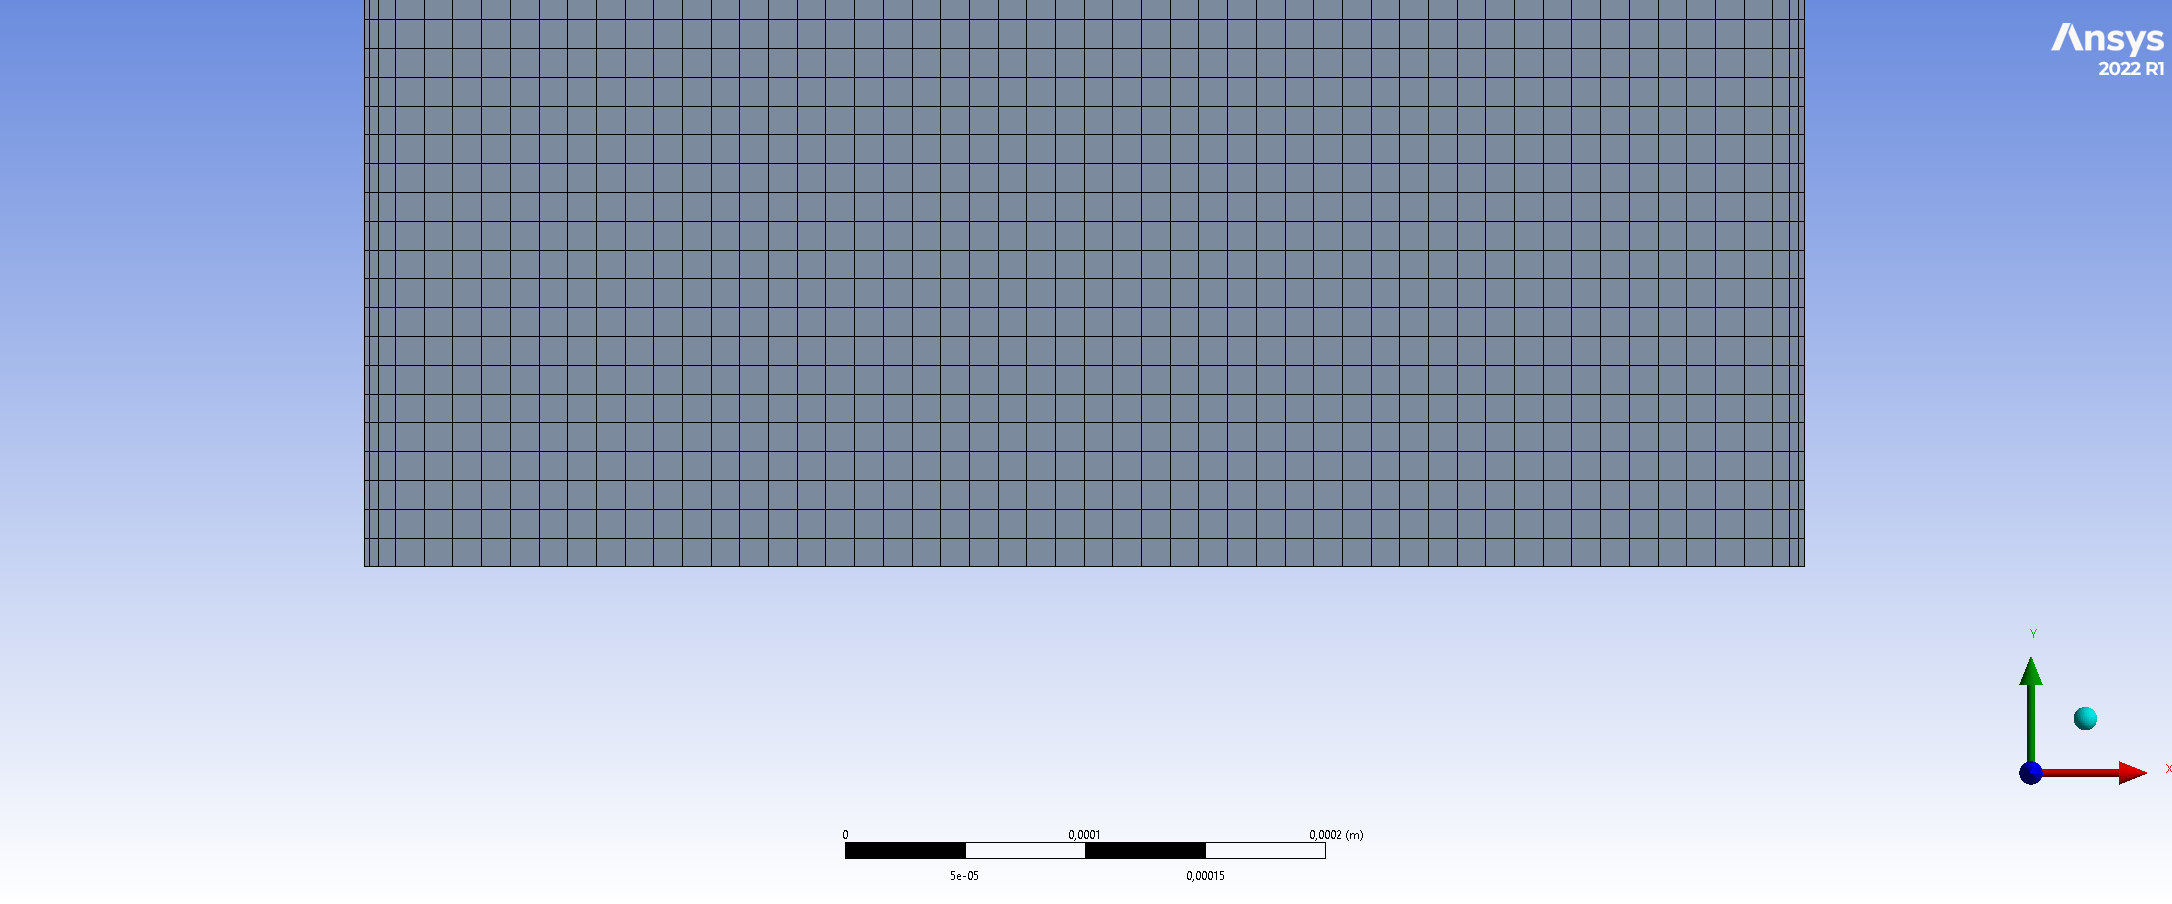
\includegraphics[scale=0.25]{Mesh}
	\caption{Ansys Meshing example}
	\label{fig:ansys_meshing}
\end{figure}
The figure shows the reactor's inlet section. The goal in meshing was to create rectangular grid out of squares or rectangles. Near the walls, that begin on the left and right side of the inlet, the mesh resolution is increased using two inflation layers. That is done to resolve the boundary layer of the flow near the walls. Having a mesh consisting mostly out of squares and rectangles is advantageous because the algorithm only stores the values at the cell's centre as mentioned in \autoref{sec:QUICK}. Having a mesh that can be seen as a 2 dimensional array makes post-processing a lot easier. How the results are extracted from the model's output will be explained in \autoref{} in greater detail.

\subsection{setup}
\label{sec: setup}

To setup the model at first a few basic configuration steps need to done. The Settings that need to be applied are listed in \autoref{tab:ansys_setup_general}.

\begin{table} [htb]
	\centering
	\caption{General settings}
	\begin{tabular}{ ccc }
		\hline
		Section & Setting & value \\
		\hline
		Solver & Type & Pressure-Based \\
		Solver & Velocity Formulation & Absolute  \\
		Solver & Time &  Transient  \\
		Solver & 2D Space & Axisymmetric \\
		\hline
		\label{tab:ansys_setup_general}
	\end{tabular}
\end{table}
With these general settings are done the used models need to be activated. The used models settings are given in \autoref{tab:ansys_setup_models}.

\begin{table} [htb]
	\centering
	\caption{model settings}
	\begin{tabular}{ cc }
		\hline
		variable & value \\
		\hline
		Energy & On \\
		Viscous & Laminar \\
		Species & (Species Transport, Reactions)  \\
		\hline
		\label{tab:ansys_setup_models}
	\end{tabular}
\end{table}

After the correct models are turned on and parametrized the species taking part within the model are defined. Within this case 4 fluids are needed. The example configuration of one of the fluids taking part within the reaction is shown in \autoref{tab:ansys_setup_materials}. The table shows the configuration of one of the educts.
\begin{table} [htb]
	\centering
	\caption{Example fluid settings}
	\begin{tabular}{ ccc }
		\hline
		variable & value & unit \\
		\hline
		density & 1000 & kg/m³ \\
		viscosity & 0.001003 & kg/(m*s) \\
		molecular weight & 100 & kg/kmol \\
		\hline
		\label{tab:ansys_setup_materials}
	\end{tabular}
\end{table}
All other values, namely enthalpies and other thermodynamic properties are the same for all the fluids and equal to the values of water. Since 3 fluids take part in the reaction and 4 fluids are needed to setup the model the yet missing fluid is water. It is needed to be able to set a molar concentration at the inlet that is lower than the maximum of 1. After this the values from the fluids should be carried over to the mixture configuration within the new existing Mixture tab. With the mixture settings the reaction parameters are set. The parameters set for the reaction are stated in \autoref{tab:ansys_setup_rection}.
\begin{table} [htb]
	\centering
	\caption{reaction settings}
	\begin{tabular}{ ccc }
		\hline
		variable & value & unit \\
		\hline
		Reaction Type & Volumetric & - \\
		Stoich. Coefficient fluid\_a & 1 & - \\
		Stoich. Coefficient fluid\_b & 1 & - \\
		Stoich. Coefficient fluid\_c & 1 & - \\
		Rate Exponent fluid\_a & 1 & - \\
		Rate Exponent fluid\_b & 1 & - \\
		Rate Exponent fluid\_c & 0 & - \\
		Pre-Exponential Factor & 1e15 & - \\
		Activation Energy & 1e4 & J/(kg*mol) \\
		\hline
		\label{tab:ansys_setup_rection}
	\end{tabular}
\end{table}
To achieve a nearly instant reaction when molecules of the two species A and B meet the rate constant which also known as Pre-Exponential Factor (see \autoref{eqn:reaction}) is set to a very high value. The Activation Energy is set to a value that the given temperature is high enough to let the reaction happen.

After the reaction is setup correctly the boundary conditions are being set. Conditions need to be set for the inlet, outlet and the walls. All information needed to configure the boundary conditions are visible in \autoref{tab:ansys_setup_boundary}

\begin{table} [htb]
	\centering
	\caption{boundary conditions}
	\begin{tabular}{ cccc }
		\hline
		place & variable & value & unit \\
		\hline
		inlet & Type & velocity-inlet & - \\
		inlet & Velocity Specification Method & Magnitude, Normal to Boundary & - \\
		inlet & Velocity Magnitude & e.g. 4e-3 & m/s \\
		inlet & Temperature & 300 & K \\
		inlet & fluid\_a & 5.4e-4 & - \\
		outlet & Type & pressure-outlet & - \\
		outlet & Gauge Pressure & 20 & Pa \\
		outlet & Prevent Reverse Flow & yes & - \\
		wall & Type & wall & - \\
		wall & Wall Motion & Stationary Wall & - \\
		wall & Shear Condition & No Slip & - \\
		\hline
		\label{tab:ansys_setup_boundary}
	\end{tabular}
\end{table}
There is a homogenous velocity profile set at the inlet normal to the boundary. At the inlet the amount of $fluid\_a$ has to set as a mole fraction as well. To get matching conditions to the already performed experiments the mole fraction needs to be calculated from a given concentration. Assuming the values from \autoref{tab:ansys_setup_molefrac} are known the mole fraction can be calculated using \autoref{eqn:molefrac}.

\begin{table} [htb]
	\centering
	\caption{needed variables for mole and mass fraction calculation}
	\begin{tabular}{ cccc }
		\hline
		variable & description & value & unit \\
		\hline
		$M_{W}$ & Molar Mass water & 18 & g/mol \\
		$M_{A}$ & Molar Mass $fluid\_a$ & 100 & g/mol \\
		$M_{fluid\_b}$ & Molar Mass $fluid\_b$ & 100 & g/mol \\
		$\rho_{water}$ & Density water & 1000 & kg/m³ \\
		$c_{fluid\_b}$ & Concentration $fluid\_b$ & 0.03 & mol/l \\
		$c_{water}$ & Concentration water & 55.55 & mol/l \\
		$Q$ & inlet flow rate &  e.g. 0.144 & ml/min \\
		\hline
		\label{tab:ansys_setup_molefrac}
	\end{tabular}
\end{table}

\begin{equation}
	\label{eqn:molefrac}
	x_{B} =\dfrac{\dot{n_{B}}}{\dot{n_{B}} + \dot{n_{W}}} = \dfrac{c_{B} \cdot Q}{c_{B} \cdot Q + c_{W} \cdot Q} = \dfrac{c_{B}}{c_{B} + c_{W}} \approx 0 \text{.}00054
\end{equation}
Since the concentration for $fluid\_{A}$ within the internal domain has to be setup as mass fraction the needed value can be calculated using \autoref{eqn:massfrac}.

\begin{equation}
	\label{eqn:massfrac}
	\varphi_{A} =\dfrac{n_{A} \cdot M_{A}}{n_{A} \cdot M_{A} + n_{W} \cdot M_{W}} = \dfrac{c_{A} \cdot M_{A}}{c_{A} \cdot M_{A} + c_{W} \cdot M_{W}} \approx \text{0.003}
\end{equation}

The temperature is set to 300 K at the inlet and within the hole internal domain. The outlet is configured to be a pressure outlet without reverse flow to get physical valid results. At the walls the usual conditions applied to walls are set with no slip and stationary.

The next step performed is to setup the solution methods as shown in \autoref{tab:ansys_setup_sol_methods}. As the solving scheme the PISO algorithm is used, that is explained in \autoref{sec:sol_method}. For spatial discretization second order methods, as explained in \autoref{sec:QUICK}, are used. 
\begin{table} [htb]
	\centering
	\caption{solution methods}
	\begin{tabular}{ ccc }
		\hline
		tab & variable & value \\
		\hline
		Pressure-Velocity Coupling & Scheme & PISO \\
		Spatial Discretization & Pressure & Second Order \\
		Spatial Discretization & Momentum & QUICK \\
		Spatial Discretization & $fluid\_a$ & Second Order Upwind \\
		Spatial Discretization & $fluid\_b$ & Second Order Upwind \\
		Spatial Discretization & $fluid\_c$ & Second Order Upwind \\
		Spatial Discretization & Energy & Second Order Upwind \\
		\hline		
		\label{tab:ansys_setup_sol_methods}
	\end{tabular}
\end{table}

The last settings that need to done before the model can be run are the time settings as shown in \autoref{tab:ansys_setup_time}. An adaptive method is chosen that is based on the CFL-Number $c$. This number can be calculated using \autoref{eqn:cfl} and is also known as Courant-Number. It is influenced by the velocity $u$, the time step $ \Delta t$ and the spacial discretization $\Delta x$. It is best practice to keep this number below or equal to 1 for stability reasons. This can be otherwise thought of as a limiting factor in a way that to rapid changes from one cell to the next one between time steps are inhibited.  
\begin{equation}
	\label{eqn:cfl}
	c = \dfrac{u \cdot \Delta t}{\Delta x}
\end{equation}
In this model the Courant number is set to 1 and the initial time step size is set to 0.01 seconds to get a compromise between simulation stability and calculation time. The time step size is updated after every calculation. The factor for time step changes are limited to 0.5 on the lower and 2 at the upper end. The time step algorithm decides for a time step change based on the Courant number. In addition to the model's time settings the interval the results are exported at need to be set. This in addition to the exported variables of interest can be set under $\texttt{Solution} \rightarrow \texttt{Activities} \rightarrow \texttt{Manage...}$.

\begin{table} [htb]
	\centering
	\caption{time settings}
	\begin{tabular}{ ccc }
		\hline
		variable & value & unit \\
		\hline
		Type & Adaptive & - \\
		Method & CFL-Based & - \\
		Duration Specification Method & Total Time & -\\
		Total Time & e.g. 20 & s \\
		Courant Number & 1 & - \\
		Fixed Timsteps & 1 & - \\
		Initial Time Step Size & 0.01 & s \\
		Max Iteration/Time Step & 30 & - \\
		Time Step Size Update Interval & 1 & - \\
		Minimum Time Step Size & e.g. 0.001 & s \\
		Maximum Time Step Size & e.g. 0.5 & s \\
		Minimum Step Change Factor & 0.5 & - \\
		Maximum Step Change Factor & 2 & - \\		
		\hline
		\label{tab:ansys_setup_time}
	\end{tabular}
\end{table}

\subsection{model evolution and refinement}

Here the steps taken to receive the final model for each case are explained.

For each of the three different reactor geometries two to three meshes are created that are shown in \autoref{tab: reactor meshes}.

\begin{table} [htb]
	\centering
	\caption{case meshes}
	\begin{tabular}{ ccc }
		\hline
		reactor height [mm] & element size [m] & mesh elements \\
		\hline
		0.2 & 6e-6 & 185000\\
		0.2 & 4e-6 & 405000\\
		0.2 & 2e-6 & 1560000\\
		0.4 & 12e-6 & 92500\\
		0.4 & 8e-6 & 202500\\
		0.4 & 4e-6 & 780000\\
		0.6 & 4e-6 & 1155154\\
		0.6 & 2e-6 & 4560304\\
		\hline		
		\label{tab: reactor meshes}
	\end{tabular}
\end{table}

Each case is run for the coarsest mesh and the results are inspected. If the Courant number field does not show values larger than 1 and the velocity field looks believable too the run is called successful. If that is not the case the next finer mesh is chosen and the case is run again. 

To be able to compare cases with each other two dimensionless numbers are chosen. First the Pecelt Number $Pe$ that can be calculated using \autoref{eqn: Pe}. This number is influenced by the reactors gap height $l$, the feed's input velocity $u$ and the mixture's Diffusion coefficient $D$.

\begin{equation}
	\label{eqn: Pe}
	Pe = \dfrac{l \cdot u}{D}
\end{equation}

The second dimensionless number chosen is the Schmidt number $Sc$. This parameter is only influenced, according to \autoref{eqn: Sc}, by the mixture's properties. $\nu$ is the viscosity and $D$ the already known diffusion coefficient.
\begin{equation}
	\label{eqn: Sc}
	Sc = \dfrac{\nu}{D}
\end{equation}

For the Peclet number 3 different values are chosen and for the Schmidt number 2 values are implemented. These values are in case of $Pe$ 500, 931 and 2050. The Schmidt number $Sc$ has either a value of 2430 or 12000. The Schmidt number mostly influences the diffusion coefficient as the viscosity $\nu$ does not change a lot between the two chosen values. Having fixed the Schmidt number and the diffusion coefficient, the Peclet number mostly influences the input velocity. An overview of the performed cases and their input variable values can be seen in \autoref{tab: cases}. Besides the reactor height $h$, the Peclet number $Pe$ and other needed input variables, the simulation time and export time in seconds need to be set. The simulation time is the physical time that represents for how long the model should be simulated. The export time sets the time interval in seconds at which results are exported during the transient simulation. These results, that contain all the values for all variables of interest for each cell, are the basis for further analysis. How the results are obtained and how they are further processed is explained in \autoref{sec: model res}.

\begin{landscape}
	\begin{table}[htb]
		\centering
		\caption{simulation cases}
		\label{tab: cases}
		\small
		\begin{tabular}{cccccccccc}
			\textbf{h [m]} & \textbf{Pe} & \textbf{Sc} & \textbf{$\nu$ [m²/s]} & \textbf{$D$ [m²/s]} & \textbf{u [m/s]} & \textbf{$x_A$} & \textbf{$\varphi_B$} & \textbf{simulation time [s]} & \textbf{export time [s]} \\
			\hline
			2.00E-04            & 500         & 2430        & 1.00E-06               & 4.11E-10               & 1.03E-03              & 5.40E-04      & 3.00E-03        & 60                            & 0.5                       \\
			2.00E-04            & 500         & 12000       & 1.20E-06               & 1.00E-10               & 2.50E-04              & 5.40E-04      & 3.00E-03        & 60                            & 0.1                       \\
			2.00E-04            & 500         & 120000      & 1.20E-06               & 1.00E-11               & 2.50E-05              & 5.40E-04      & 3.00E-03        & 60                            & 0.1                       \\
			2.00E-04            & 931         & 2430        & 1.00E-06               & 4.11E-10               & 1.91E-03              & 5.40E-04      & 3.00E-03        & 60                            & 0.5                       \\
			2.00E-04            & 931         & 12000       & 1.20E-06               & 1.00E-10               & 4.66E-04              & 5.40E-04      & 3.00E-03        & 60                            & 0.1                       \\
			2.00E-04            & 931         & 120000      & 1.20E-06               & 1.00E-11               & 4.66E-05              & 5.40E-04      & 3.00E-03        & 60                            & 0.1                       \\
			2.00E-04            & 2050        & 2430        & 1.00E-06               & 4.11E-10               & 4.21E-03              & 5.40E-04      & 3.00E-03        & 60                            & 0.5                       \\
			2.00E-04            & 2050        & 12000       & 1.20E-06               & 1.00E-10               & 1.02E-03              & 5.40E-04      & 3.00E-03        & 60                            & 0.1                       \\
			2.00E-04            & 2050        & 120000      & 1.20E-06               & 1.00E-11               & 1.02E-04              & 5.40E-04      & 3.00E-03        & 60                            & 0.1                       \\
			4.00E-04            & 500         & 2430        & 1.00E-06               & 4.11E-10               & 5.14E-04              & 5.40E-04      & 3.00E-03        & 60                            & 0.5                       \\
			4.00E-04            & 500         & 12000       & 1.20E-06               & 1.00E-10               & 1.25E-04              & 5.40E-04      & 3.00E-03        & 60                            & 0.1                       \\
			4.00E-04            & 500         & 120000      & 1.20E-06               & 1.00E-11               & 1.25E-05              & 5.40E-04      & 3.00E-03        & 60                            & 0.1                       \\
			4.00E-04            & 931         & 12000       & 1.20E-06               & 1.00E-10               & 2.33E-04              & 5.40E-04      & 3.00E-03        & 60                            & 0.1                       \\
			4.00E-04            & 931         & 2430        & 1.00E-06               & 4.11E-10               & 9.57E-04              & 5.40E-04      & 3.00E-03        & 60                            & 0.5                       \\
			4.00E-04            & 931         & 120000      & 1.20E-06               & 1.00E-11               & 2.33E-05              & 5.40E-04      & 3.00E-03        & 60                            & 0.1                       \\
			4.00E-04            & 2050        & 12000       & 1.20E-06               & 1.00E-10               & 5.12E-04              & 5.40E-04      & 3.00E-03        & 60                            & 0.5                       \\
			4.00E-04            & 2050        & 2430        & 1.00E-06               & 4.11E-10               & 2.10E-03              & 5.40E-04      & 3.00E-03        & 60                            & 0.5                       \\
			4.00E-04            & 2050        & 120000      & 1.20E-06               & 1.00E-11               & 5.12E-05              & 5.40E-04      & 3.00E-03        & 60                            & 0.1                       \\
			6.00E-04            & 500         & 2430        & 1.00E-06               & 4.11E-10               & 3.43E-04              & 5.40E-04      & 3.00E-03        & 60                            & 0.5                       \\
			6.00E-04            & 500         & 12000       & 1.20E-06               & 1.00E-10               & 8.33E-05              & 5.40E-04      & 3.00E-03        & 60                            & 0.5                       \\
			6.00E-04            & 500         & 120000      & 1.20E-06               & 1.00E-11               & 8.33E-06              & 5.40E-04      & 3.00E-03        & 60                            & 0.5                       \\
			6.00E-04            & 931         & 12000       & 1.20E-06               & 1.00E-10               & 1.55E-04              & 5.40E-04      & 3.00E-03        & 60                            & 0.5                       \\
			6.00E-04            & 931         & 2430        & 1.00E-06               & 4.11E-10               & 6.38E-04              & 5.40E-04      & 3.00E-03        & 60                            & 0.5                       \\
			6.00E-04            & 931         & 120000      & 1.20E-06               & 1.00E-11               & 1.55E-05              & 5.40E-04      & 3.00E-03        & 60                            & 0.5                       \\
			6.00E-04            & 2050        & 12000       & 1.20E-06               & 1.00E-10               & 3.41E-05              & 5.40E-04      & 3.00E-03        & 60                            & 0.5                       \\
			6.00E-04            & 2050        & 2430        & 1.00E-06               & 4.11E-10               & 1.40E-03              & 5.40E-04      & 3.00E-03        & 60                            & 0.5                       \\
			6.00E-04            & 2050        & 120000      & 1.20E-06               & 1.00E-11               & 3.41E-05              & 5.40E-04      & 3.00E-03        & 60                            & 0.5						\\
			\hline      
		\end{tabular}
	\end{table}
\end{landscape}

\subsection{model implementation}

In this part the model implementation and execution is explained.

When having to run a model for a variety of sets of input values it is useful to think about reducing the manual performed steps to a minimum. This has the advantages to provide a scaleable solution if the set of input variables increases or the number of different values that need to be looked at grows. When having to set large amount of variables at different places within the model manually, the process is prone to errors that might not be detected until the results are computed or in case of small ones are not detected at all.

In general the developed solution follows the guideline shown in \autoref{fig: software_guideline}.

\begin{figure}[htbp]
	\centering
	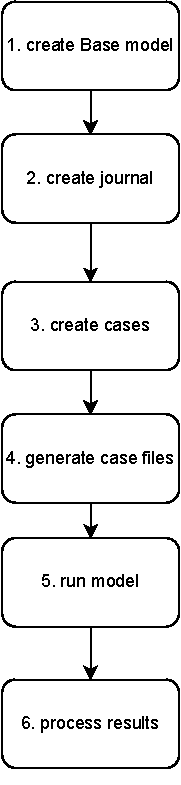
\includegraphics[scale=1.0]{software_proc}
	\caption{implementation guideline}
	\label{fig: software_guideline}
\end{figure}

The first step that needs to be done when creating a set of cases is the creation of a base model. This step mostly includes the geometry creation and meshing. It is important that the results exported, that are directly influenced by the mesh are able to be further processed. That is why the mesh in this work's base models mostly consists out of squares and rectangles. The creation of the base model is done using the tool \texttt{ANSYS WORKBENCH}.

The next step is to create a journal that sets all the values for the input variables. The file is called journal according to \cite{manual2009ansys} and is used to automate \texttt{ANSYS FLUENT} model execution. This journal can easily be created by using the build in macro recording tool of \texttt{ANSYS FLUENT}. Within this journal all needed settings that are not already set within the base model itself must be included. A part of such a journal is shown in \autoref{lst: journal}. One of the last steps of such a journal is the export of a model and a data file to a target location chosen by the user. This step is needed when looking into parallel execution of models that will be explained later.

%\lstinputlisting[language=Bash, caption=journal example]{code/testjournal.jou} 
%\lstinputlisting[caption=journal example, label=lst: journal]{code/testjournal.jou}

\definecolor{codehighlight}{rgb}{0.95,0.8,0.8}
\lstinputlisting[caption=journal example, label=lst: journal, basicstyle=\fontsize{9}{10}\selectfont\ttfamily, linebackgroundcolor={%
	\ifnum\value{lstnumber}=3\color{yellow!40}\fi 
	\ifnum\value{lstnumber}=7\color{yellow!40}\fi    
	\ifnum\value{lstnumber}=8\color{yellow!40}\fi
	\ifnum\value{lstnumber}=13\color{yellow!40}\fi
}
]{code/testjournal.jou}

From the highlighted lines in \autoref{lst: journal} it can be seen that for each variable that needs to be set by the journal a variable name is defined and put between to two \% signs for easier identification. With this approach new variables can be efficiently added. When the journal is created by the user and the journal functionality is tested and proven the cases need to be created. A case is defined here as one model execution with a set of input parameters and their values. The cases can be created in different ways but need to be provided in .json format in the end. An example of such a case in correct format can be seen in \autoref{lst: case}. The file providing the cases can contain as many as needed. 

\lstinputlisting[caption=case example, label=lst: case, basicstyle=\fontsize{9}{10}\selectfont\ttfamily]{code/testcase.json}

After the cases are provided and all previous steps are done as well all cases can be created by running the developed tool \texttt{journal.py}.
This tool creates a folder for each case at the destination provided within \texttt{conf.json} and creates all files needed to execute the case. This script needs to be run on a machine that has \texttt{ANSYS FLUENT} installed and is able to write to the desired destination. The version used here is \texttt{Fluent 2022 R1}. Having all files needed for case execution within the case's folder makes parallel case execution possible because cases have no cross referenced files. That also helps with developing, debugging and checking the case at future times, as all things necessary are there.

If all cases are created successfully they can be run in parallel on an High Performance Computing (HPC) Cluster. The journal template files developed within this work also provide a variant for local execution but that is not recommended when having a large amount of cases to run and if the number of cells get rather high. Since a HPC Cluster was used here this work focuses on that execution variant.

\begin{figure}[htbp]
	\centering
	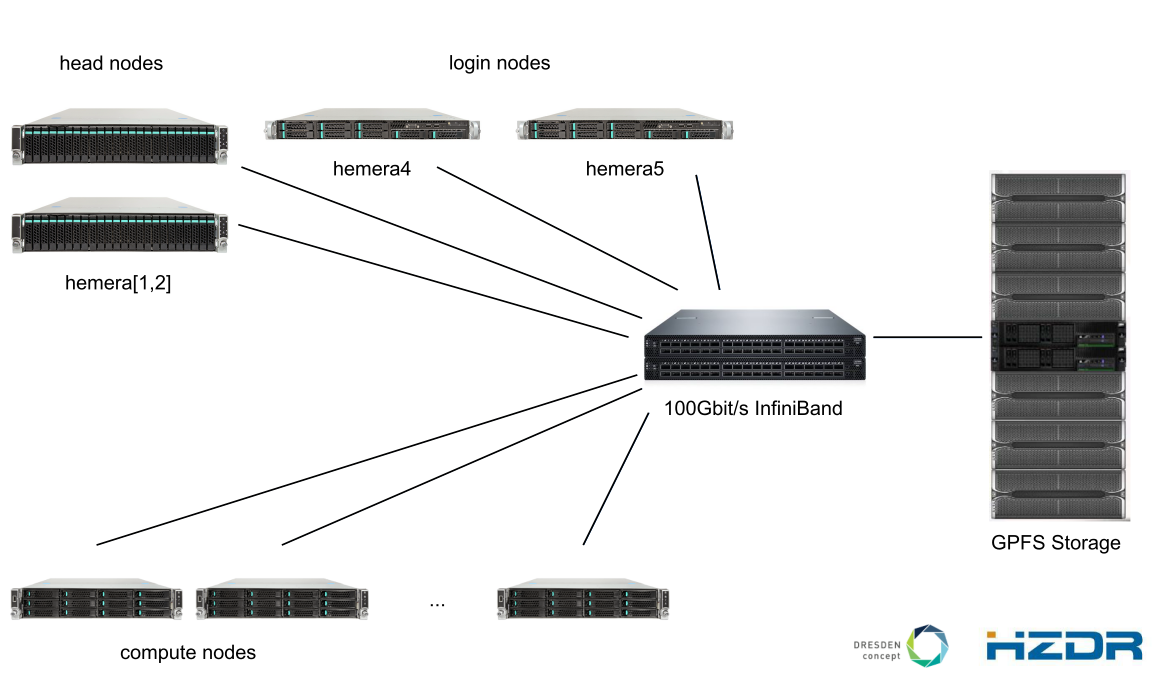
\includegraphics[scale=0.5]{HPC_Cluster}
	\caption{HPC Cluster Overview}
	\label{fig: HPC_Cluster}
\end{figure}

A brief overview of the Cluster used is provided in \autoref{fig: HPC_Cluster} \cite{schulz2022hardware_and_num}. A Cluster usually consists of 5 different components. To provide a high amount of computational power compute nodes are needed. This can be as many as rack space and or other limiting factors are available. To feed the compute nodes with calculations to perform the head nodes are doing the load balancing. A task that needs to be performed on the cluster is called job. These jobs are created on the login nodes and then submitted to the head nodes that run a queueing system. The one used here is \texttt{slurm}. For data and storage access all nodes are connected to a storage server using an industry standard high capacity network connection. It is not wise to run the login and head nodes on the same piece of hardware as one could think because if the head nodes crash the hole cluster becomes inoperable. To minimise this risk these two tasks are separated onto different machines.

For the queueing system \texttt{slurm} to accept a job a few parameters need to be set. Each job needs to have a partition and wall time set. The partition refers to a given queue on the cluster. There are different queues for different purposes and not all of them are available to each user.
The wall time is needed to set the maximum time a job is allowed to run. This prevents failing jobs to block the cluster for an infinite time. In addition to these two parameters, as shown in \autoref{lst: case} the hardware requirements of a job need to be set. This is the amount of nodes the job needs and the amount of CPUs that are reserved on each node. Since \texttt{ANSYS FLUENT} calculations can not be distributed over more than one node the amount of nodes is always 1. The CPU Cores used can be in a range of 1 to the maximum the hardware bound to the chosen queue has to offer. Higher demand of resources in combination with long wall times might lead to high queueing times so it is worth spending a thought on them. When having cluster access the developed script \texttt{run.sh} can be run with the option \texttt{-a} to run all jobs that have not generated any data. After some time has passed the script \texttt{time\_estat.py} can be run to get a estimation of the remaining job runtime using \autoref{eqn: rem_runtime}. The script will also warn the user if the set wall time is lower than the estimated execution time. The tool grabs the current job execution status out of the simulation's log file and uses the current job run time to calculate the total and remaining execution time. 
\begin{equation}
	\label{eqn: rem_runtime}
	t_{exec,remain} = \underbrace{\dfrac{t_{sim,total}}{t_{sim,current}} \cdot t_{exec,current}}_{\text{total execution time}}  - t_{exec,current} 
\end{equation}
These values can be easily compared with the set wall time.    

\end{document}